\section{Component Diagram}
Nella figura \ref{fig:ComponentDiagram_iterazione3} è riportato il diagramma a componenti dell'applicazione dove sono state evidenziate le interfacce inserite nell'iterazione 3. 
\begin{figure}[h!]
	\centering
	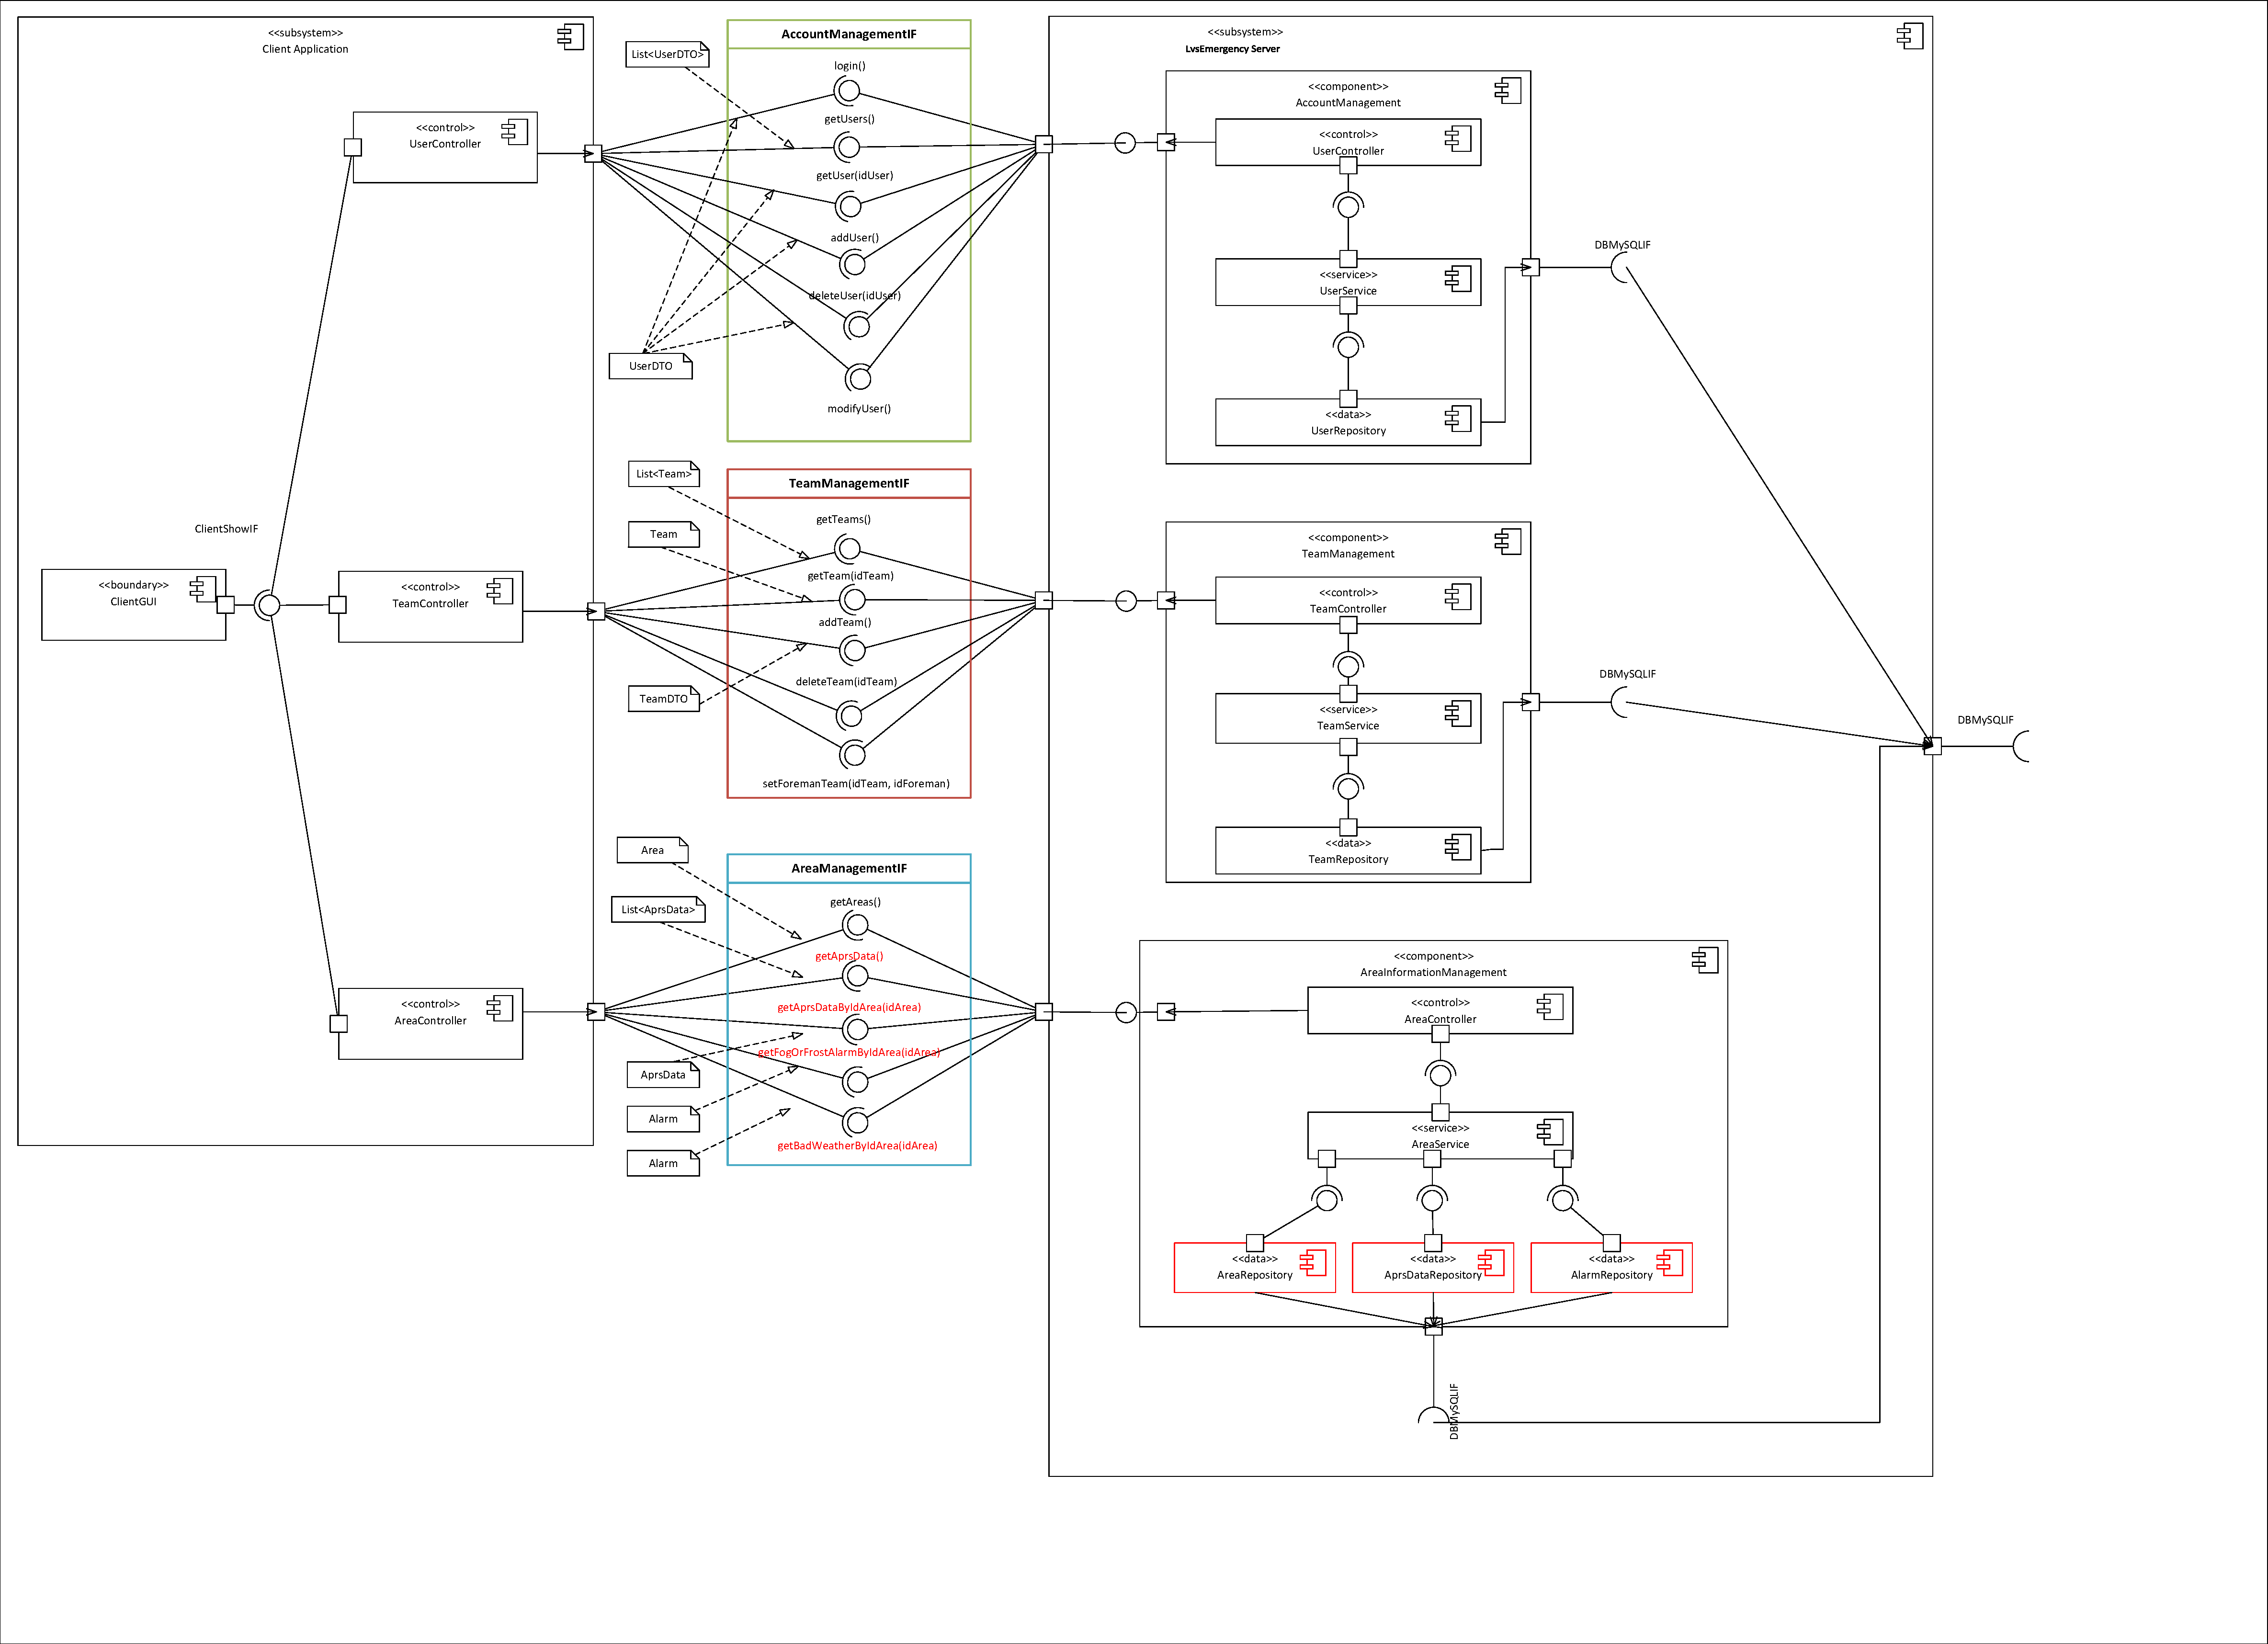
\includegraphics[width=1\linewidth]{./Iterazione 3/OtherFiles/UML - Component view}
	\caption{Component Diagram.}
	\label{fig:ComponentDiagram_iterazione3}
\end{figure}

\clearpage

\section{Interface and Packages Diagram}
Le API implementate in questa iterazione sono state inserite nel package \textit{AreaInformationManagement} (\Fig\ref{fig:InterfaceDiagram_iterazione3}) e sono gestite dall'\textit{Area Controller}.

\begin{figure}[h!]
	\centering
	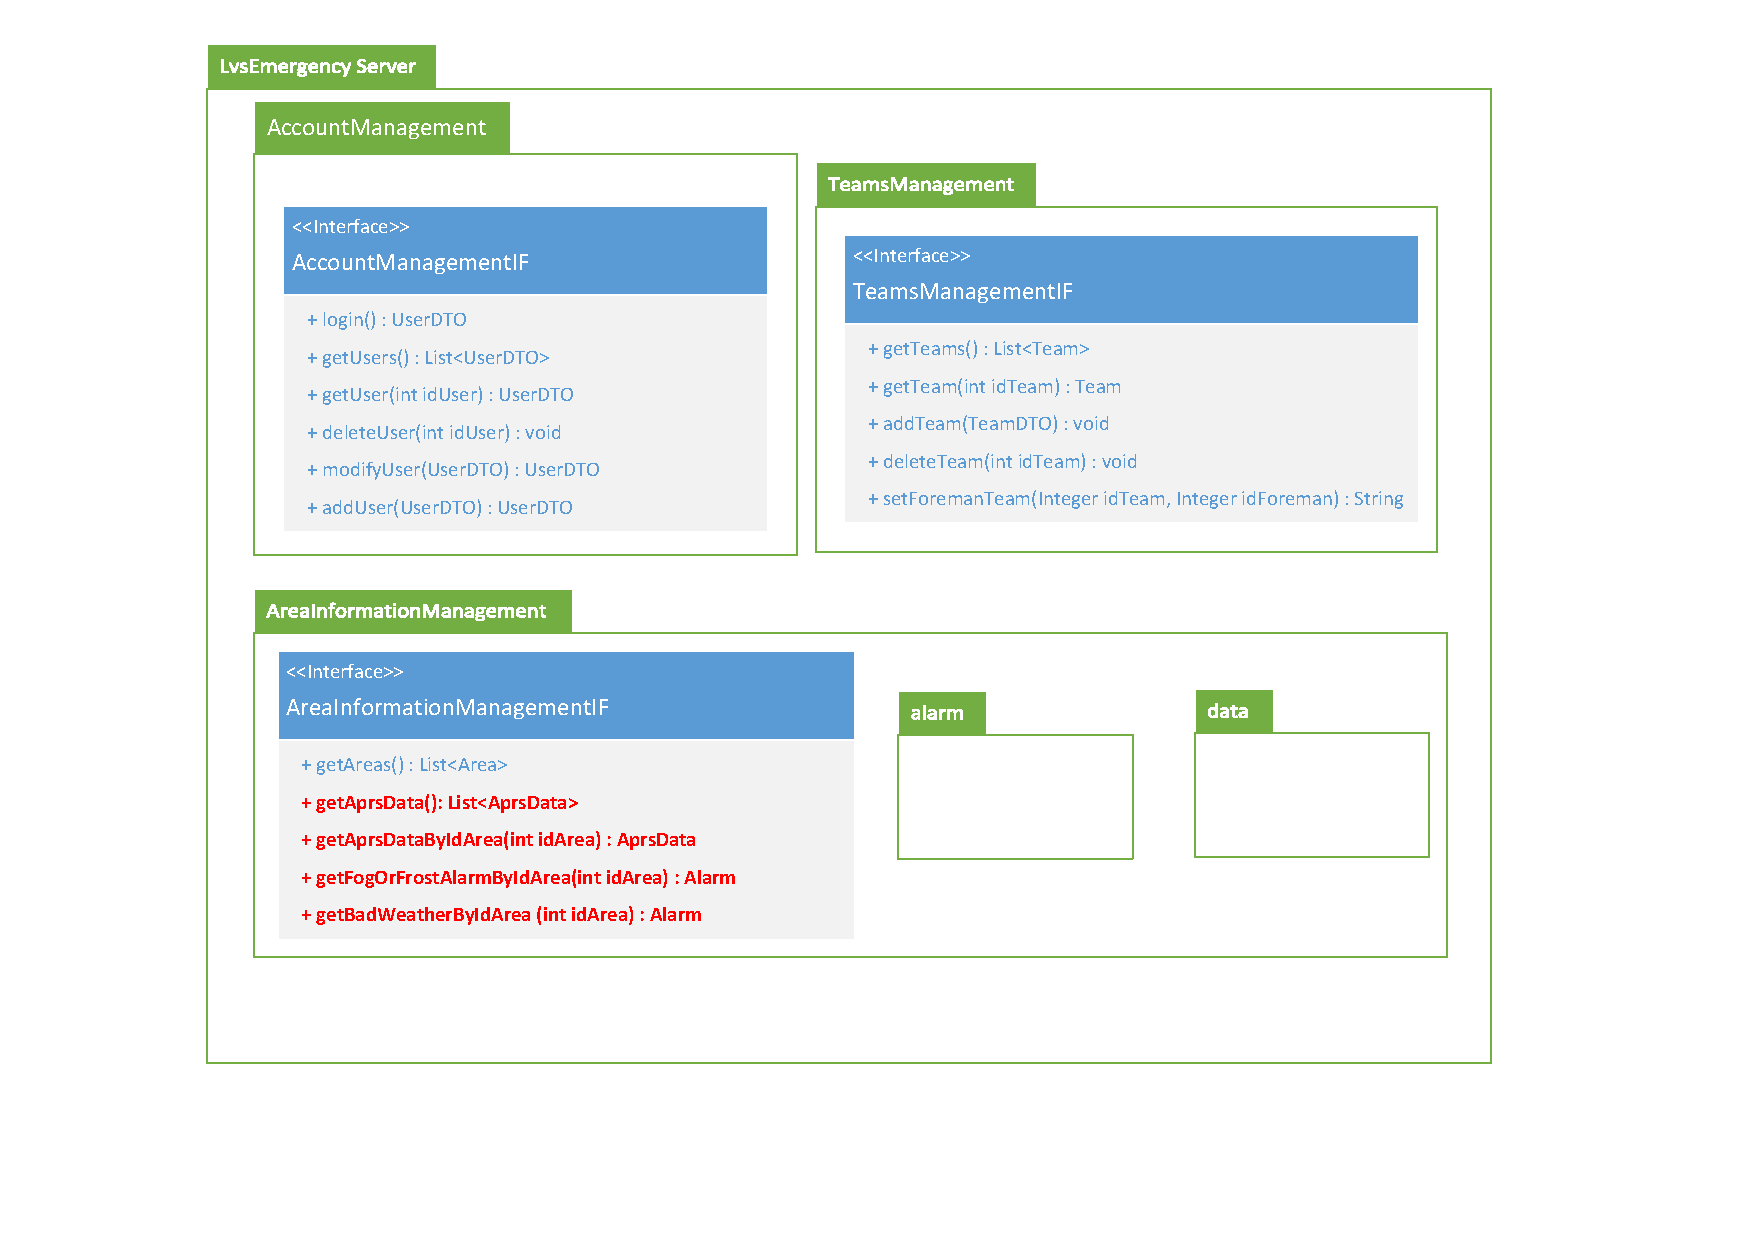
\includegraphics[width=0.8\linewidth]{./Iterazione 3/OtherFiles/UML - Interface Diagram}
	\caption{Interface and Package Diagram.}
\label{fig:InterfaceDiagram_iterazione3}
\end{figure}